\documentclass{beamer}
\usetheme{sintef}

\newcommand{\testcolor}[1]{\colorbox{#1}{\textcolor{#1}{test}}~\texttt{#1}}

\usepackage{amsfonts,amsmath,oldgerm}
\usefonttheme[onlymath]{serif}

%------------------------------------------------

\usepackage{booktabs} % Required for better table rules
\usepackage{listings} % For writing code
\usepackage{pgfgantt} % For building grantt charts
\usepackage{mathabx}
\usepackage{graphicx}
% \usepackage{subcaption}
\usepackage{tabularx}
\usepackage{verbatim}
\usepackage{subfig}
\usepackage{xcolor}
\usepackage{caption}
\usepackage{tikz}
\usepackage{mathtools}
\usepackage{pgfplots}
\usepackage{amssymb}

% Command for timeline entry
% \newcommand{\ytl}[2]{%
%   \colorbox{gray}{\begin{tabular}{@{}p{0.2\linewidth}@{\hspace{4pt}}p{0.7\linewidth}@{}}%
%       \raggedleft #1 & #2
%   \end{tabular}}\vspace{4pt}}

\newsavebox{\measurebox}
\lstset{
    language=C,
    basicstyle=\ttfamily,
    keywordstyle=\color{blue},
    commentstyle=\color{green},
    stringstyle=\color{red},
    showstringspaces=false,
    breaklines=true
}

%----------------------------------------------------------------------------------------
%	 TITLE SLIDE
%----------------------------------------------------------------------------------------

\titlebackground*{Assets/ppt/GAUHATI}

\newcommand{\hrefcol}[2]{\textcolor{cyan}{\href{#1}{#2}}}

\title{Seminar On \\ \vspace{0.5ex}SEMINAR TITLE}

\author{\large{Author Name}}
% \institute{}

% \IDnumber{PS-811-211-0006}

% \course{\small{Supervisor}: \normalsize{Dr.\ Irani Hazarika }}

\institute{hhhh}

\date{29 September 2023}

%------------------------------------------------

\begin{document}

%------------------------------------------------

\maketitle
%------------------------------------------------

%----------------------------------------------------------------------------------------
%	 HEADER PAGE
%----------------------------------------------------------------------------------------

% \begin{frame}

% This template is a based on \hrefcol{https://www.overleaf.com/latex/templates/sintef-presentation/jhbhdffczpnx}{SINTEF Presentation} from \hrefcol{mailto:federico.zenith@sintef.no}{Federico Zenith} and its derivation \hrefcol{https://github.com/TOB-KNPOB/Beamer-LaTeX-Themes}{Beamer-LaTeX-Themes} from Liu Qilong

% \vspace{\baselineskip}

% In the following you find a brief introduction on how to use \LaTeX\ and the beamer package to prepare slides, based on the one written by \hrefcol{mailto:federico.zenith@sintef.no}{Federico Zenith} for \hrefcol{https://www.overleaf.com/latex/templates/sintef-presentation/jhbhdffczpnx}{SINTEF Presentation}

% % This template is released under \hrefcol{https://creativecommons.org/licenses/by-nc/4.0/legalcode}{Creative Commons CC BY 4.0} license

% \end{frame}
%------------------------------------------------

%----------------------------------------------------------------------------------------
%	 SECTION 0
%----------------------------------------------------------------------------------------

% \section{Introduction}

% \input{MainSlides/Finsec0.tex}
\section{CHAPTER 1}
\begin{chapter}[Assets/ppt/GAUHATIw]{}{Chapter 1}
    \begin{enumerate}
        \item Section 1
        \item Section 2
        \item Section 3
    \end{enumerate}
\end{chapter}

% \begin{sidepic}{images/svm/svm.png}{SVM}

% \end{sidepic}

% \begin{textimg}{What is SVM?}{images/svm/svm.png}
% ddd
% \end{textimg}

\begin{frame}{What?}
    \begin{columns}
        \begin{column}{0.45\textwidth}
            A linear classifier which seeks to find a seperating plane which is at a maximum distance from both feature sets.
        \end{column}
        \begin{column}{0.45\textwidth}
            \begin{figure}
                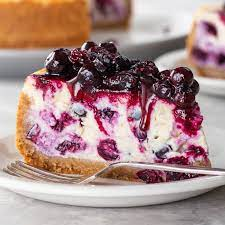
\includegraphics[height=\textheight]{Images/bbc.jpeg}
            \end{figure}
        \end{column}
    \end{columns}
\end{frame}


\section{CHAPTER 2}
% \section{Multiclass SVM}

\begin{chapter}[Assets/ppt/GAUHATIw]{}{Chapter 2}
    \begin{itemize}
        \item Section 1
        \item Section 2
        \item Section 3
    \end{itemize}
\end{chapter}

% \begin{sidepic}{Assets/ppt/GAUHATI}{jjj}

% \end{sidepic}

\begin{frame}{AA}
    \begin{columns}
        \begin{column}{0.5\textwidth}

        \end{column}
        \begin{column}{0.5\textwidth}

        \end{column}
    \end{columns}
\end{frame}



\begin{frame}{TITLE}

    \[ \mathbf{S} = \mathbf{W} \cdot \mathbf{X} \]

    So, for any $\omega_j$ in $\omega$ $$\omega_j \cdot x_i + \omega_0 = S_j $$

    This means that for the input vector $X_i$, a score component $S_j$ gives the score of $\omega_j$.

\end{frame}

% \begin{frame}{Score function of Linear Machine}
%     dd
% \end{frame}


% \section{Optimizing Loss Function}
% \begin{chapter}[Assets/ppt/GAUHATIw]{}{Multi-class Linear Classification}

% \end{chapter}
%------------------------------------------------


%------------------------------------------------
\backmatter
\end{document}
